%%%%start parameter to change
\def\assignmentnum{2}
\def\assignmenttitle{XCS251 Assignment \assignmentnum : Perform Bitcoin transactions using python-bitcoinlib}
\def\month{September}
\def\weekday{Sunday}
\def\day{25}
\def\time{11:59pm}
\def\postquestion{slack channel}
\def\submissiononline{Gradescope}
\def\latextemplate{assigment2-template.tex}

%%%%end parameter to change

\def\due{Due \weekday, \month\ \day\ at \time\ PT.}




\documentclass[11pt]{article}
\usepackage{epsfig,amsfonts,amsmath,amssymb,graphics,fullpage}

\usepackage{epsfig,amsfonts,amsmath,amssymb,graphics,fullpage,xcolor}
\usepackage[colorlinks=true,linkcolor=blue,urlcolor=blue, citecolor=blue, hidelinks]{hyperref}
\hypersetup{colorlinks=true,citecolor=blue,linkcolor=blue,linktocpage=true}
\DeclareUrlCommand\url{\color{blue}}


\newcommand{\comment}[1]{}
\newcommand{\deq}{\mathrel{:=}}
\newcommand{\cat}{\mathrel{\|}}
\newcommand{\KK}{\mathcal{K}}  % key space
\newcommand{\XX}{\mathcal{X}}   % input space
\newcommand{\YY}{\mathcal{Y}}   % output space
\newcommand{\MM}{\mathcal{M}}   % output space
\newcommand{\CC}{\mathcal{C}}   % output space
\newcommand{\CIPHER}{\mathcal{E}}   % cipher

\setlength{\topmargin}{0in}
\setlength{\headheight}{0in}
\setlength{\headsep}{0in}
\setlength{\topskip}{0in}

\newcommand{\lcat}{\langle}
\newcommand{\rcat}{\rangle}
\newcommand{\tuple}[1]{\lcat #1 \rcat}

\newcommand{\DES}{{\sf DES}}

\newcommand{\xor}{\oplus}
\newcommand{\Z}{\mathbb{Z}}
\newcommand{\adv}{\mathcal{A}}
\newcommand{\bdv}{\mathcal{B}}
\newcommand{\rgets}{\stackrel{\scriptscriptstyle{R}}{\leftarrow}}
\newcommand{\EXP}{\textrm{EXP}}


\newenvironment{myalg}{\begin{list}{}{
        \setlength{\labelwidth}{0.5cm}
        \setlength{\leftmargin}{1cm}
        \setlength{\itemsep}{0cm}
        \setlength{\topsep}{0cm}
        \setlength{\parsep}{0.05cm}}}{\end{list}}

\newcommand{\squish}{
      \setlength{\topsep}{0pt}
      \setlength{\itemsep}{0ex}
      \vspace{-1ex}
      \setlength{\parskip}{0.05cm}}
\newcommand{\squishend}{\vskip -1ex\relax}

%\newcommand{\solution}[1]{\noindent{\bf Solution:} {\it {#1}}}
\newcommand{\solution}[1]{}


%%%%%%%%
\usepackage{color}
\usepackage{ulem}
\usepackage{hyperref} % for URL links
\usepackage{amsmath} % for cases environment

%%%%%%%%


\usepackage{enumitem}
\newenvironment{problems}
{\begin{enumerate}[label=\bfseries Exercise \arabic*.,align=left]}
{\end{enumerate}}

\newenvironment{subparts}
{\begin{enumerate}[label=\bfseries \alph*.,align=right,leftmargin=1.5em]}
{\end{enumerate}}
%%%%%%%%
\usepackage[headsep=1cm,headheight=2cm]{geometry}
\usepackage{fancyhdr}
\pagestyle{fancy}
%%
%%
\lhead{\assignmenttitle}
\rhead{\thepage}
\cfoot{}
%%
\renewcommand{\headrulewidth}{0pt}
\renewcommand{\footrulewidth}{0pt}
\newcommand{\ruleskip}{\bigskip\hrule\bigskip}
\newcommand{\latex}{\LaTeX\xspace}
\newcommand{\Hint}{\noindent {\bf Hint: }}
\setlength\parindent{0pt}

\begin{document}

{\Huge\assignmenttitle}

\ruleskip


{\bf \due}

\vspace{0.2cm}
{\bf Guidelines}
\begin{enumerate}[itemsep=2pt]
    \item If you have a question about this assignment, we encourage you to post your question on \postquestion.
    \item Familiarize yourself with the collaboration and honor code policy before starting work.
\end{enumerate}

\vspace{0.2cm}

{\bf Submission Instructions} 
\vspace{0.2cm}

You should submit a PDF with your solutions online in \submissiononline. As long as the PDF is legible and
organized, the course staff has no preference between a handwritten and a typeset \LaTeX{} submission. If you wish
to typeset your submission and are new to \LaTeX{}, you can get started with the following:

\begin{itemize}
    \item Download and install \href{https://www.tug.org/texlive/}{Tex Live} or try \href{https://www.overleaf.com/}{Overleaf}.
    \item Submit the compiled PDF.
\end{itemize}

\vspace{0.2cm}

{\bf Honor code} 
\vspace{0.2cm}

We strongly encourage students to form study groups. Students may discuss and
work on assignment in groups. However, each student must write down the
solutions independently, and without referring to written notes from the joint
session. In other words, each student must understand the solution well enough
in order to reconstruct it by him/herself. In addition, each student should
write on the assignment the set of people with whom s/he collaborated. Further,
because we occasionally reuse problem set questions from previous years, we
expect students not to copy, refer to, or look at the solutions in preparing
their answers. It is an honor code violation to intentionally refer to a
previous year's solutions.  More information regarding the Stanford honor code
can be found at \href{https://communitystandards.stanford.edu/policies-and-guidance/honor-code}{https://communitystandards.stanford.edu/policies-and-guidance/honor-code}.

\vspace{0.2cm}

\newpage
{\bf Introduction} 
\vspace{0.2cm}

\sloppy
In this assignment, you will gain experience creating transactions using the Bitcoin and BlockCypher testnet blockchains and Bitcoin Script. This assignment consists of four questions, and the starter code we provide uses python-bitcoinlib, a free, low-level Python 3 library for manipulating Bitcoin transactions. Details on the background of bitcoin transaction and testnet, the instructions on getting started with the started code, and setup steps to interact with the Bitcoin testnet will be provided in the handout. By the end of this assignment, you should have a good understanding of how Bitcoin transactions work.

\vspace{0.2cm}

\section{Project Background}

\subsection{Anatomy of a Bitcoin Transaction}
\begin{figure}[h!]
  \centering
  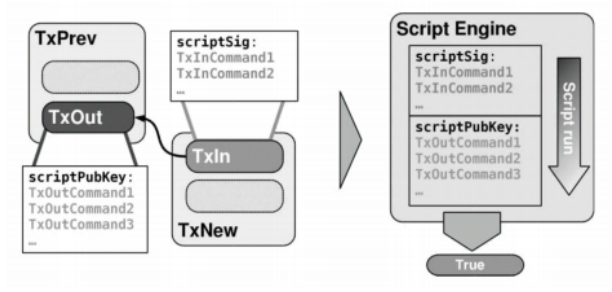
\includegraphics[width=.75\textwidth]{txin_txout.png}
  \caption{Each \texttt{TxIn} references the \texttt{TxOut} of a previous
    transaction, and a \texttt{TxIn} is only valid if its scriptSig outputs
  True when prepended to the \texttt{TxOut}'s scriptPubKey.}
\label{figure:txin_txout}
\end{figure}

\hspace{20pt} Bitcoin transactions are fundamentally a list of outputs, each of which is associated with an amount of bitcoin that is ``locked'' with a puzzle in the form of a program called a scriptPubKey (also sometimes called a ``smart contract''), and a list of inputs, each of which references an output from the list of outputs and includes the ``answer'' to that output's puzzle in the form of a program called a scriptSig.
Validating a scriptSig consists of appending the associated scriptPubKey to it, running the combined script and ensuring that it outputs True.

\[
  \text{run}(\textbf{scriptSig } || \textbf{ scriptPK}) =
  \begin{cases}
      \text{True} & \text{valid scriptSig, TxIn spend TxOut} \\
      \text{else} & \text{invalid scriptSig, TxIn cannot spend TxOut}
   \end{cases}
\]

\hspace{20pt} Most transactions are ``PayToPublicKeyHash'' or ``P2PKH'' transactions, where the scriptSig is a list of the recipient's public key and signature, and the scriptPubKey performs cryptographic checks on those values to ensure that the public key hashes to the recipient's bitcoin address and the signature is valid.

\hspace{20pt} Each transaction input is referred to as a \texttt{TxIn}, and each transaction output is referred to as a \texttt{TxOut}. The situation for a transaction with a single input and single output is summarized by Figure \ref{figure:txin_txout} above.

\hspace{20pt}The sum of the bitcoin in the unspent outputs to a transaction must not exceed the sum of the inputs for the transaction to be valid. The difference between the total input and total output is implicitly taken to be a transaction fee, as a miner can modify a received transaction and add an output to their address to make up the difference before including it in a block.

\[\sum \text{TxIn} = \sum \text{TxOut} + \text{Tx}_{\text{fee}}\]

\hspace{20pt}For the first 3 questions in this project, the transactions you create will consume one input and create one PayToPublicKeyHash output that sends an amount of bitcoin back to the testnet faucet. The 4th question will carry out a swap of coins between two entities, Alice and Bob. For these exercises, you will want to take the fee into account when specifying how much to send and subtract a bit from the amount in the output you're sending, say 0.001 BTC (this is just to be safe, you can probably include a fee as low as 0.00001 BTC if your funds are running low). \textcolor{blue}{If you do not include a fee, it is likely that your transaction will never be added to the blockchain. Since BlockCypher (see Section~\ref{testnets}) will delete transactions that remain unconfirmed after a day or two, it is very important that you include a fee to make sure that your transactions are eventually confirmed.}

\subsection{Script Opcodes}
Your code will use the Bitcoin stack machine's opcodes, which are documented on the Bitcoin wiki [1]. When composing programs for your transactions' scriptPubKeys and scriptSigs you may specify opcodes by using their names verbatim. For example, below is an example of a function that returns a scriptPubKey that cannot be spent, but rather acts as storage space for an arbitrary piece of data that someone may want to save to the blockchain using the \texttt{OP\_RETURN} opcode.
\begin{verbatim}
    def save_message_scriptPubKey(message):
        return [OP_RETURN,
                message]
\end{verbatim}

\hspace{20pt}Examples of some opcodes that you will likely be making use of include \texttt{OP\_DUP}, \texttt{OP\_CHECKSIG}, \texttt{OP\_EQUALVERIFY}, and \texttt{OP\_CHECKMULTISIG}, but you will end up using additional ones as well.

\subsection{Overview of Testnets} {\label{testnets}}
Rather than having you download the entire testnet blockchain and run a bitcoin client on your machine, we will be making use of an online block explorer to upload and view transactions. The one that we will be using is called BlockCypher, which features a nice web interface as well as an API for submitting raw transactions that the starter code uses to broadcast the transactions you create for the exercises. After completing and running the code for each exercise, BlockCypher will return a JSON representation of your newly created transaction, which will be printed to your terminal. An example transaction object along with the meaning of each field can be found at BlockCypher's developer API documentation at 
\href{https://www.blockcypher.com/dev/bitcoin/\#tx}{https://www.blockcypher.com/dev/bitcoin/\#tx}.
Of particular interest for the purposes of this project will be the \texttt{hash}, \texttt{inputs}, and \texttt{outputs} fields. Note that you will be using two different test networks (``testnets'') for this project: the Bitcoin testnet (the current version is Testnet3) for questions 1-4 and the BlockCypher testnet for question 4. These will be useful in testing your code. As part of these exercises, you will request coins to some addresses (more details below).

\section{Getting Started}
\begin{enumerate}
\item Download the starter code, navigate to the directory, create and activate python virtual environment and run \texttt{pip install -r requirements.txt} to intall the required dependencies. For this project, \textcolor{blue}{ensure that you are using Python 3.} You can type \texttt{python --version} to find out if you are using Python 3 under \texttt{python} command. You can type \texttt{pip --version} to find out if you are using Python 3 under \texttt{pip} command. To create, activate, and deactivate a Python virtual environment, check \href{https://packaging.python.org/en/latest/tutorials/installing-packages/#creating-virtual-environments}{https://packaging.python.org/en/latest/tutorials/installing-packages/\#creating-virtual-environments}. If you are not using a Python virtual environment, you must do two things differently. First, use \texttt{pip3} instead of \texttt{pip} to install packages to Python 3. Second, use the \texttt{python3} command to run scripts instead of \texttt{python} to run with the Python 3 interpreter.




\item Make sure you understand the structure of Bitcoin transactions and read the references in the Recommended Reading section \ref{sec:rreading} if you would like more information.

\item Read over the starter code. Recommend the use of an IDE for simplicity. Visual Studio Code or PyCharm are excellent.
Here is a summary of what each of the files contain:
    \subitem \texttt{lib/keygen.py}:
    \subitem You will run this script to generate new private keys and corresponding addresses for the Bitcoin Testnet. Questions 1-3 will solely use these private keys, while question 4 will also require you to use an alternative method to generate Block Cypher Testnet keys. \textbf{You are not expected to modify this file.}
    \vspace{0.3cm}
    \subitem \texttt{lib/split\_test\_coins.py}:
    \subitem You will run this script to split your coins across multiple unspent transaction outputs (UTXOs). You will have to edit this file to input details about which transaction output you are splitting, the UTXO index, etc.
    \vspace{0.3cm}
    \subitem \texttt{lib/config.py}:
    \subitem You will modify this file to include the private keys for your users. Note that \texttt{my\_private\_key}, \texttt{alice\_secret\_key\_BTC} and \texttt{bob\_secret\_key\_BTC} will be generated using the \texttt{lib/keygen.py} file. You will make web requests to generate \texttt{alice\_secret\_key\_BCY} and \texttt{bob\_secret\_key\_BCY}. \textbf{There are comments in \texttt{config.py} and instructions during setup for how to do this}.
    \vspace{0.3cm}
    \subitem \texttt{lib/utils.py}:
    \subitem Contains various util methods. \textbf{You are not expected to modify this file.}
    \vspace{0.3cm}
    \subitem \texttt{Q1.py, Q2a.y, Q2b.py, Q3a.py, Q3b.py, Q4.py}:
    \subitem You will have to modify the various scriptSig and scriptPubKey methods, as well as fill the transaction parameters. Note that for question 3, you will have to generate additional private and public keys for customers using the \texttt{lib/keygen.py} file.
    \vspace{0.3cm}
    \subitem \texttt{alice.py, bob.py}:
    \subitem Creates and submits transactions for Q4 on behalf of Alice and Bob. \textbf{You are not expected to modify these files.}
    \vspace{0.3cm}
    \subitem \texttt{swap.py}
    \subitem Contains the logic to carry out the atomic swap. \textbf{You are not expected to modify this file.}
    \vspace{0.3cm}
    \subitem \texttt{docs/transactions.py}
    \subitem You are expected to fill this file with the transaction ids generated for questions 1-3.
    \vspace{0.3cm}
    \subitem \texttt{docs/Q4design\_doc.txt}
    \subitem You are expected to fill this design doc to explain your solution to Q4.

\item Be sure to start early on this project, as block confirmation times can vary depending on how busy the network is!

\end{enumerate}


\section{Setup}
\begin{enumerate}
    \item Open \texttt{lib/config.py} and read the file. Note that there are several users that you will need to generate private keys and addresses for.
    \item First we are going to generate key pairs for you, Alice, and Bob on the Bitcoin Testnet. Run \texttt{lib/keygen.py} to generate private keys for \texttt{my\_private\_key}, \texttt{alice\_secret\_key\_BTC} and \texttt{bob\_secret\_key\_BTC}, and record these keys in \texttt{lib/config.py}. Note that Alice and Bob's keys will only come into play for question 4. Please make sure to create different keys for Alice and Bob, you wouldn't want them to be able to forge each others' transactions! You may want to record each generated private key and address in a separate file and note the corresponding user for easy reference.
    \item Next, we want to get some test coins for \texttt{my\_private\_key} and  \texttt{alice\_secret\_key\_BTC}. To do so: \begin{enumerate}
        \item Go to the Bitcoin Testnet faucet
        (\href{https://testnet-faucet.mempool.co/}{https://testnet-faucet.mempool.co/}) and paste in the corresponding addresses of the users.
        Note that faucets will often rate-limit requests for coins based on Bitcoin address and IP address, so try not to lose your test Bitcoin too often. It is recommended that you use the address associated with \texttt{my\_private\_key} with the first faucet listed above since that faucet gives more coins and you will be performing more exercises with that address. Note that the faucet limits requests by the same IP address to  max 0.002 per hour and 0.002  per request. Therefore, use lesser amount for each address to avoid max out.


        \item You may want to record the transaction hash, i.e., TxID, in the same file that you record the generated private key and address for each user. An example screenshot is provided in Figure \ref{figure:txid} below.

\begin{figure}[h!]

  \centering
  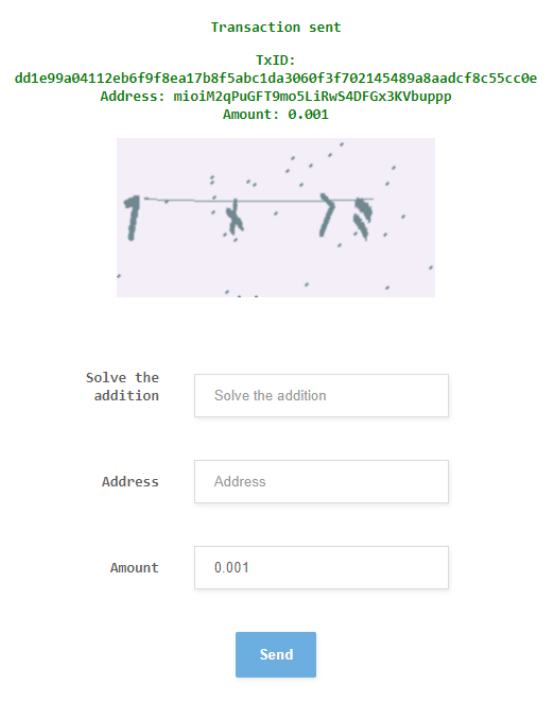
\includegraphics[width=.75\textwidth]{txid.png}
  \caption{Screenshot of TxID.}
\label{figure:txid}
\end{figure}


Viewing the transaction in a block explorer (e.g.
        \href{https://live.blockcypher.com/}{https://live.blockcypher.com/}) will also let you know which output of the transaction corresponds to your address, and you will need this \texttt{utxo\_index} for the next step as well.  For example, if you search the address that you just requested a coin in Bitcoin Testnet, you can see the transaction with the TxID in Figure \ref{figure:transcation} below. 

\begin{figure}[h!]

  \centering
  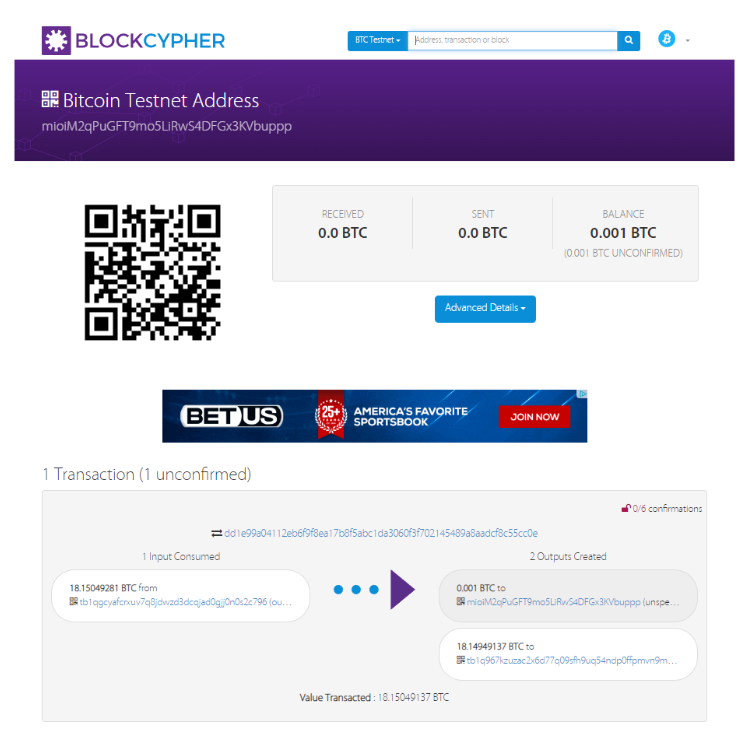
\includegraphics[width=.75\textwidth]{transcation.png}
  \caption{Screenshot of Transaction.}
\label{figure:transcation}
\end{figure}

Requested value 0.001 is the first output, i.e., \texttt{utxo\_index} 0. If it is the second output, then it will be \texttt{utxo\_index} 1. You will also see “0/6 confirmations”. You will want to wait for fully verified (at least 6/6 confirmations) to split the coin as described in step 6.

If the faucet doesn't give you a transaction hash, you can also paste the user address into the block explorer and find the transaction that way. It is best to navigate the blocks using the user address if the transaction hash does not work.
    \end{enumerate}
    \item Next, we are going to create generate key pairs for Alice and Bob on the BlockCypher testnet.
    \begin{enumerate}
		\item
			Sign up for an account with Blockcypher to get an API token here: \\
			\href{https://accounts.blockcypher.com/}{https://accounts.blockcypher.com/} \\
			You need a valid email to confirm the account. Please save the new token in a text file for future reference.
		\item
			Create BCY testnet keys for Alice and Bob and place into \texttt{lib/config.py}.
			\begin{verbatim}
  		curl -X POST 'https://api.blockcypher.com/v1/bcy/test/addrs?token=YOURTOKEN'
			\end{verbatim}
    		Note, if you copy this command directly into your terminal from this handout, you'll likely need to delete and retype the \verb|'| for the command to work. Also note that for Windows OS, you will want to use double quote rather than single quote like below

                       \begin{verbatim}
  		curl -X POST "https://api.blockcypher.com/v1/bcy/test/addrs?token=YOURTOKEN"
			\end{verbatim}
		Remember to record the results in a separate file like before and note the corresponding user for easy reference 

	\end{enumerate}
	\item
		Give Bob's address bitcoin on the Blockcypher testnet (BCY) and record the transaction hash.
		\begin{verbatim}
		curl -d '{"address": "BOBS_BCY_ADDRESS", "amount": 100000}' \
		'https://api.blockcypher.com/v1/bcy/test/faucet?token=YOURTOKEN'
		\end{verbatim}
		Note, if you copy this command directly into your terminal from this handout, you'll likely need to delete and retype the \verb|'{| and the \verb|}'|, delete the \verb|\|, retype the \verb|'| around the url, and condense the command into one line for it to work. It is preferred to type the command to avoid reformatting issues. Also note that for Windows OS, you will want to use double quote rather than single quote.

    \item The faucets will give you, Alice, and Bob one spendable output per person, but we would like to have multiple outputs to spend in case we accidentally lock some with invalid scripts. Edit the parameters at the bottom of \texttt{split\_test\_coins.py}, where \texttt{txid\_to\_spend} is the transaction hash from the faucet to your address, \texttt{utxo\_index} is 0 if your output was first in the faucet transaction and 1 if it was second as described before, and \texttt{n} is the number of outputs you want your test coins split evenly into, and run the program with \texttt{python split\_test\_coins.py}. A perfect run through of questions 1-3 would require \texttt{n} = 3 for your address, one for each exercise, but if you anticipate accidentally locking an output due to a faulty script a couple times per exercise then you might want to set \texttt{n} to something higher like 8 so that you don't have to wait to access the faucet again or have to try with a different Bitcoin address. \textbf{If \texttt{split\_test\_coins.py} was successful, you should get back some information about the transaction.} Record the entire result with the transaction hash in a separate file like before, as each exercise will be spending an output from this transaction and will refer to it using this hash.
    
    Note: The faucet transaction would need to be fully verified (at least 6/6 confirmations) before you can split the coins you received. Waiting times will vary based on how busy the network is.
    
    \item You should also split Alice's and Bob's coins into multiple outputs just to be safe. Record the entire result in a separate file like before. Note that each time you switch between the Bitcoin and BlockCypher tesntets, you should adjust the \texttt{network\_type} variable in \texttt{lib/config.py}. Also note that in \texttt{split\_test\_coins.py}, parameters like private key in Bitcoin or BlockCyper testnets  in \texttt{config.py} are already imported. Check those imported parameters at the beginning of \texttt{split\_test\_coins.py} and select corresponding parameters to put them at the end of \texttt{split\_test\_coins.py}.

    \item At the end, verify that you created Bitcoin Testnet addresses for you,  Alice, and Bob in a block explorer (e.g. \href{https://live.blockcypher.com/}{https://live.blockcypher.com/} and select Bitcoin testnet). You and Alice should have some coins on this blockchain. There should also be BlockCypher Testnet addresses for Alice and Bob. Bob should have some coins on this blockchain. You can check by using a block explorer (e.g. \href{https://live.blockcypher.com/}{https://live.blockcypher.com/}  and select BlockCypher Testnet). If you record all the results properly in a separate file as suggested in the previous step, you should have no problem finding the corresponding address of a user in a specific testnet. Give yourself a pat on the back for finishing a long setup. Now it's time to explore creating transactions with Bitcoin Script.
\end{enumerate}

\section{Questions}
For each of the questions below, you will use the Bitcoin Script opcodes to create transactions. For question 4, you will write an atomic swap transaction across two different blockchains. To publish each transaction created for the exercises, edit the parameters at the bottom of the file to specify which transaction output the solution should be run with along with the amount to send in the transaction. If the scripts you write aren't valid, an exception will be thrown before they're published. For questions 1-3, make sure to record the transaction hash of the created transaction and write it to \texttt{docs/transactions.py}. After completing each exercise, look up the transaction hash in a blockchain explorer to verify whether the transaction was picked up by the network, i.e., finalized with 6+ confirmations. Make sure that all your transactions have been posted successfully before submitting their hashes.
\begin{problems}

\item
  Open \texttt{Q1.py} and complete the scripts labelled with \texttt{TODO}s
  to redeem an output you own and send it back to the faucet with a standard
  PayToPublicKeyHash transaction. The faucet address is already included in the starter code for you. Your functions should return a list consisting of only OP codes and parameters passed into the function.

\item For question 2, we will generate a transaction that is dependent on some constants.
    \begin{enumerate}
        \item Open \texttt{Q2a.py}. Generate a transaction that can be redeemed by the solution $(x,y)$ to the following system of two linear equations:
        \[
            x+y = \text{(YYYY, which is your birthday year)}  \qquad\text{and}
	\]
	\[
            x-y = \text{(MMDD, which is your birthday month and day without leading zero)}
        \]

	For an integer solution to exist, the rightmost digit of your birthday year and your birthday month and day must either be both even or both odd. Therefore, you can change the rightmost digit of your birthday month and day to match the evenness or oddness of the rightmost digit of your birthday year.
For example, if your birthday is January 1st, 2000. Then $x+y = 2000$ and $x - y = 101$. Now, to match even and oddness, change 101 to 102, so you have $x+y = 2000$ and $x-y = 102$. You then have an integer solution $x= 1051$ and $y= 949$.  Make sure you use \texttt{OP\_ADD} and \texttt{OP\_SUB} in your scriptPubKey.
        \item Open \texttt{Q2b.py}. Redeem the transaction you generated above. The redemption script should be as small as possible. That is, a valid scriptSig should consist of simply pushing two integers $x$ and $y$ to the stack.
    \end{enumerate}

\item Next, we will create a multi-sig transaction involving four parties.
    \begin{enumerate}
        \item Open \texttt{Q3a.py}. Generate a multi-sig transaction involving four parties such that the transaction can be redeemed by the first party (bank) combined with any one of the 3 others (customers) but not by only the customers or only the bank. \textcolor{blue}{You may assume the role of the bank for this problem so that the bank's private key is your private key and the bank's public key is your public key. Generate the customers' keys using \texttt{lib/keygen.py} and paste them in \texttt{Q3a.py}.}
        \item Open \texttt{Q3b.py}. Redeem the transaction and make sure that the scriptSig is as small as possible. You can use any legal combination of signatures to redeem the transaction but make sure that all combinations would have worked. Specifically, make sure that bank’s signature plus any customer’s signature should redeem the transaction. You do not need to worry about the case when multiple customers' signatures are provided. You can design the order of the signatures anyway you want as long as it can redeem the transaction. 
    \end{enumerate}

\item Last but not least, you will create a transaction called a {\it cross-chain atomic swap}, allowing two entities to securely trade ownership over cryptocurrencies on different blockchains. In this case, Alice and Bob will swap coins between the Bitcoin testnet and BlockCypher testnet. As you recall from setup, Alice has bitcoin on BTC Testnet3, and Bob has bitcoin on the BCY Testnet. They want to trade ownership of their respective coins securely, something that can't be done with a simple transaction because they are on different blockchains. The idea here is to set up transactions around a secret x, that only one party (Alice) knows. In these transactions only H(x) will be published, leaving x secret. Transactions will be set up in such a way that once x is revealed, both parties can redeem the coins sent by the other party. If x is never revealed, both parties will be able to retrieve their original coins safely, without help from the other. Before you start, make sure to read \texttt{swap.py}, \texttt{alice.py}, and \texttt{bob.py}. Compare to the pseudocode in \href{https://en.bitcoin.it/wiki/Atomic\_cross-chain\_trading}{https://en.bitcoin.it/wiki/Atomic\_cross-chain\_trading}. This will be very helpful in understanding this assignment. Note that for this question, you will only be editing \texttt{Q4.py} and you can test your code by running \texttt{python swap.py}.

    \begin{enumerate}
    \item
    	Consider the ScriptPubKey necessary for creating a transaction to carry out a cross-chain atomic swap. This transaction must be redeemable by the recipient (if they have a secret x that corresponds to Hash(x)), or redeemable with signatures from both the sender and the recipient. Write this ScriptPubKey in coinExchangeScript in \texttt{Q4.py}.

    \item Write the accompanying ScriptSigs:
    	\begin{enumerate}
    	\item
    		Write the ScriptSig necessary to redeem the transaction in the case where the recipient knows the secret x. Write this in coinExchangeScriptSig1 in \texttt{Q4.py}.
    	\item
    		Write the ScriptSig necessary to redeem the transaction in the case where both the sender and the recipient sign the transaction. Write this in coinExchangeScriptSig2 in \texttt{Q4.py}.
    	\end{enumerate}
    \item
    	Run your code using \texttt{python swap.py}. We aren't requiring that the transactions be broadcasted, as that requires some waiting to validate transactions. Running with broadcast\_transactions=False will validate that ScriptSig + ScriptPK return true. Try this for alice\_redeems=True as well as alice\_redeems=False.

    	\textbf{OPTIONAL:} Try with broadcast\_transactions=True, which will make the code sleep for an appropriate amount of time to post everything to the blockchain and verify correctly. Warning: will take 30 or more minutes to run.
    \item Fill in \texttt{docs/Q4design\_doc.txt} with the following information:
        \begin{enumerate}
            \item An explanation of what you wrote and how the coinExchangeScript works.
            \item Briefly, how the coinExchangeScript you wrote fits into the bigger
            picture of this atomic swap.
            \item Consider the case of Alice sending coins to Bob with coinExchangeScript:
                \begin{itemize}
                    \item Why can Alice always get her money back if Bob doesn't redeem it?
                    \item Why can't this be solved with a simple 1-of-2 multisig?
                \end{itemize}
            
        \end{enumerate}

    \end{enumerate}
\end{problems}

\section{Submitting your code}
Record your transaction hashes in the \texttt{docs/transactions.py} file for questions 1-3. The hashes should be listed one per line in the same order as the questions.

\hspace{20pt}For question 4, make sure \texttt{docs/Q4design\_doc.txt} is filled out and your code verifies when run with \texttt{broadcast\_transactions=False}.

\hspace{20pt}Please submit all code for this assignment. Please create a single .tar or .zip file that includes all your deliverables for all four questions. Submit via Gradescope.

\section{FAQ and tips}

\begin{enumerate}
\item When you run \texttt{keygen.py} during setup, you may encounter the following libeay32 issue in the error message. 

\begin{verbatim}
FileNotFoundError: Could not find module 'libeay32' (or one of its 
dependencies). Try using the full path with constructor syntax. 
\end{verbatim}

This seems to happen in Windows OS very often. The reason is  that the following command \texttt{\_ssl = ctypes.cdll.LoadLibrary(ctypes.util.find\_library('ssl') or 'libeay32')} in \texttt{key.py} can not find \texttt{libeay32}. 

For Windows OS, one fix used by some students in the past is to directly download \texttt{libeay32} in \texttt{openssl-1.0.2d-x64\_86-win64.zip}  from \href{https://indy.fulgan.com/SSL/Archive/}{https://indy.fulgan.com/SSL/Archive/}. Then add \texttt{libeay32.dll} to System32 folder directly. 

Another fix used by some students in the past is to install anaconda and use conda environment. First, install anaconda \href{https://www.anaconda.com/products/distribution}{https://www.anaconda.com/products/distribution}. Anaconda includes conda. Then create and activate conda environment using \texttt{conda create -n myenv python=3.9}, then \texttt{conda init cmd.exe}, and \texttt{conda activate myenv}. For details, see \href{https://docs.conda.io/projects/conda/en/latest/user-guide/tasks/manage-environments.html}{https://docs.conda.io/projects/conda/en/latest/user-guide/tasks/manage-environments.html}. Finally, do \texttt{pip install -r requirements.txt}.


\item You can check recommended reading \ref{reference:bscript} for the available opcodes. You should not use the opcodes that are disabled because miners will reject the script with disabled opcodes. 

\item In general, you should provide a reasonable transaction fee because the transaction fee may determine the priority. You can find current fee estimates on BlockCypher's block explorer below:

BTC Testnet: \href{https://live.blockcypher.com/btc-testnet/}{https://live.blockcypher.com/btc-testnet/}

BCY Testnet: \href{https://live.blockcypher.com/bcy/}{https://live.blockcypher.com/bcy/}

\item At the end of the script, the top of the stack must be 1 or True. Hence,  if you consume the last value, it won't work. See the following quote in recommended reading \ref{reference:bscript}  \texttt{A transaction is valid if nothing in the combined script triggers failure and the top stack item is True (non-zero) when the script exits.}

\item It is a good practice to verify that your scripts are fully correct before you submit a transaction. This means that when the proper inputs are provided, the script should terminate with only one item on the stack, and that item should be True. The following link provides visualization of bitcoin script execution, which may be useful. 
\href{https://siminchen.github.io/bitcoinIDE/build/editor.html}{https://siminchen.github.io/bitcoinIDE/build/editor.html}

\item Negative numbers can go into the stack. The python encoding of an integer should be able to be pushed onto the stack with no extra work from you, even if it's negative.

\item For problem 3(b), you should have a shorter script if you use  \texttt{OP\_CHECKMULTISIG} somewhere in the  \texttt{ScriptPK}.

\item f you mess up the UTXO order (could be 0 or 1 if you have two outputs), then you may have the following error message)
\begin{verbatim}
400 Bad Request
{"error": "Error validating transaction: witness script detected 
in tx without witness data."}
\end{verbatim}

\item
In the past, there were questions regarding what is being asked for the writeup in 4(d). Further elaboration is provided below. 
\begin{enumerate}
\item[i] What does your code do? How does it implement the specification we set out for you? 
\item[ii] Look through the atomic swap protocol on the \href{https://en.bitcoin.it/wiki/Atomic_swap}{wiki}. What part(s) of the protocol does your code represent? What does the code you wrote do in the protocol and why is it necessary?
\item[iii] Why can Alice always get her money back if Bob does not comply with the protocol? You may discuss the entire protocol, not just the part you implemented yourself. Why can't Alice instead issue a 1-out-of-2 multisig with her and Bob's public keys and use this transaction to get a refund if Bob does not comply instead of the existing mechanism? 
\end{enumerate}
\end{enumerate}


\section{Recommended Reading}
\label{sec:rreading}
\begin{enumerate}
  \item \label{reference:bscript}Bitcoin Script:
  \href{https://en.bitcoin.it/wiki/Script}{https://en.bitcoin.it/wiki/Script}
  \item Bitcoin Transaction Format:
  \href{https://en.bitcoin.it/wiki/Transaction}{https://en.bitcoin.it/wiki/Transaction}
  \item Bitcoin Transaction Details:
  \href{https://privatekeys.org/2018/04/17/anatomy-of-a-bitcoin-transaction/}{https://privatekeys.org/2018/04/17/anatomy-of-a-bitcoin-transaction/}
  \item How Atomic Swap Works: \href{https://en.bitcoin.it/wiki/Atomic\_cross-chain\_trading}{https://en.bitcoin.it/wiki/Atomic\_cross-chain\_trading}
\end{enumerate}
\end{document}
